\documentclass[a4,german]{article}

\usepackage[german]{babel} % für deutsche Silbentrennung und generierte Texte
\usepackage[T1]{fontenc}    % für deutsche Umlaute etc. in der Ausgabe
\usepackage[utf8]{inputenc} % für deutsche Umlaute.
\usepackage{graphicx}       % um Bilder einzubinden
\usepackage{subfigure} 	    % um 2 Bilder nebeneinander haben zu können
\usepackage{hyperref}       % um URLs korrekt einzubinden und Hyperlinks im Dokument zu ermöglichen
\usepackage{cite}
\usepackage{babelbib}


\begin{document}

\title{Cloud Computing mal anders: Klassifikation von Wolkenbildern mit kNN und CNNs}
\author{Maximilian Birkenhagen, Ali Ebrahimi, Thilo Fryen, Lukas Hintze}
\maketitle

\begin{abstract}
    Wir vergleichen zwei Ansätze zur Klassifizierung von Wolken anhand von Bildern:
        einerseits einen \glqq klassischen\grqq\ Ansatz, in dem auf Grundlage von manuell ausgewählten Merkmalen eine \emph{$k$-nearest-neighbor}-Klassifika\-tion durchgeführt wird;
        andererseits einen auf \emph{Machine Learning} basierendem Ansatz, in dem die Klassifizierung durch ein neuronales Netz auf Grundlage von von einem vortrainierten \emph{Convolutional Neural Network} extrahierten Merkmalen klassifiziert werden.
    Wir kommen zum Schluss, dass letzterer Ansatz deutlich besser geeignet ist, aber in beiden Varianten noch Potential für weitere Verbesserungen vorhanden ist.
\end{abstract}

\section{Einleitung}

Im 19. Jahrhundert begannen Wissenschaftler damit, Wolken zu typisieren, und schufen damit die Grundlage der heutigen Forschung. % TODO: Quelle?
\glqq Wolken sind ein wesentlicher Bestandteil der Atmosphäre. [...] Sie sind außerordentlich typische Kennzeichen der jeweiligen Wetterlage und Vorzeichen für die künftige Wetterentwicklung.\grqq\cite{wolkenatlas:Karlsruhe}
Daher ist die Klassifikation von Wolken nicht nur für Wolken-Enthusiasten interessant, sondern spielt auch eine große Rolle bei der Klimaforschung, Wettervorhersagen und Unwetterwarnungen.
Deshalb handelt sich bei dieser Arbeit, um das Thema Wolkenklassifizierung mit Hilfe von Bilder.

Allerdings werden bei der heutigen Bestimmung andere Messmethoden wie Radar, Laser (z.B. LiDAR) oder Radiometer präferiert, bei denen Messungen von Sensoren an verschiedenen Orten (Satellit, Bodenstationen) miteinander kombiniert werden \cite{wang}.
Es gab aber auch schon zuvor Versuche, nur mit Hilfe von Bildern Wolken zu klassifizieren:
Forscher der Universität Kiel fotografierten den gesamten Himmel immer wieder von derselben Position aus und unterschieden dabei sieben verschiedene Wolkenarten(kombinationen), darunter auch den \glqq leeren Himmel\grqq.
Mithilfe eines k-nearest-neighbour Klassifikators erreichten sie eine Genauigkeit von 97\% \cite{heinle}.
% TODO: Hier stand mal was mit Leave-One-Out Cross-Validation... ich habe es raus genommen, denn zumindest ich habe *null* Ahnung was das bedeuten soll... --Lukas


\subsection{Unsere Arbeit}

In dieser Arbeit versuchen wir, Wolken automatisiert zu klassifizieren, und vergleichen dabei zwei unterschiedliche Ansätze:
der eine Ansatz basiert auf \glqq klassischen\grqq\ Methoden der Computer Vision, das heißt auf händisch ausgewählten Merkmalen wie Mittelwert, Standardabweichung, Farb-Histogrammen und Kantenerkennung, auf deren Grundlage dann ein k-nearest-neighbor-Klassifikator angewendet wird.
Der andere basiert auf den \glqq moderneren\grqq\ Convolutional Neural Networks (CNN), die Merkmale extrahieren, auf deren Grundlagen dann die weitere Klassifikation durch ein konventionelles neuronales Netz stattfindet.


\subsection{Aufbau der Arbeit}

In Abschnitt \ref{sec:daten} erläutern wir die Daten, die unserer Arbeit zugrunde liegen, also deren Herkunft, deren Charakteristika und unsere Klasseneinteilung.
In Abschnitt \ref{sec:methodik} folgt die Darlegung unserer Klassifizierungsmethodik, in der auf die Details sowohl des klassischen als auch des auf Machine Learning basierenden Ansatzes eingegangen wird.
Abschließend werden beide Ansätze in Abschnitt \ref{sec:experimente} evaluiert und auf quantitativer Ebene verglichen, dabei erfolgt auch ein Vergleich mit der Leistung einer (kleinen) Gruppe von (nicht fachkundigen) Menschen.
Unser Fazit ist in Abschnitt \ref{sec:fazit} dargestellt.


\section{Daten}
\label{sec:daten}

Unser Datensatz besteht aus 833 Farbbildern, die zu ungefähr gleichen Teilen vom Wolkenatlas der Webseite wolken-online.de \cite{wolkenonline} und der Bildergalerie des \emph{International Cloud Atlas} der \emph{World Meteorological Organization} \cite{wmo:images} stammen.
Die Bilder sind meist von individuellen Personen geschossene Fotos vom Himmel.
Allerdings ist auf den Bildern oft nicht nur der Himmel zu sehen, sondern auch vor allem am unteren Rand die Erdoberfläche mitsamt Objekten wie Häusern oder Bäumen.
Außerdem sind gelegentlich mehrere Wolkenarten auf demselben Bild vertreten.

Der \textit{International Cloud Atlas}\cite{internationalCloudAtlas} unterscheidet zehn Wolkengattungen, welche in Abbildung~\ref{fig:cloudtypes} schematisch dargestellt sind.
Die Wolkenarten unterscheiden sich im Wesentlichen durch ihre Struktur, Dichte und Höhe, wobei die letzten beiden Eigenschaften auf Bildern nur schwer bis gar nicht erkennbar sind.

\begin{figure}[h!]
\centering
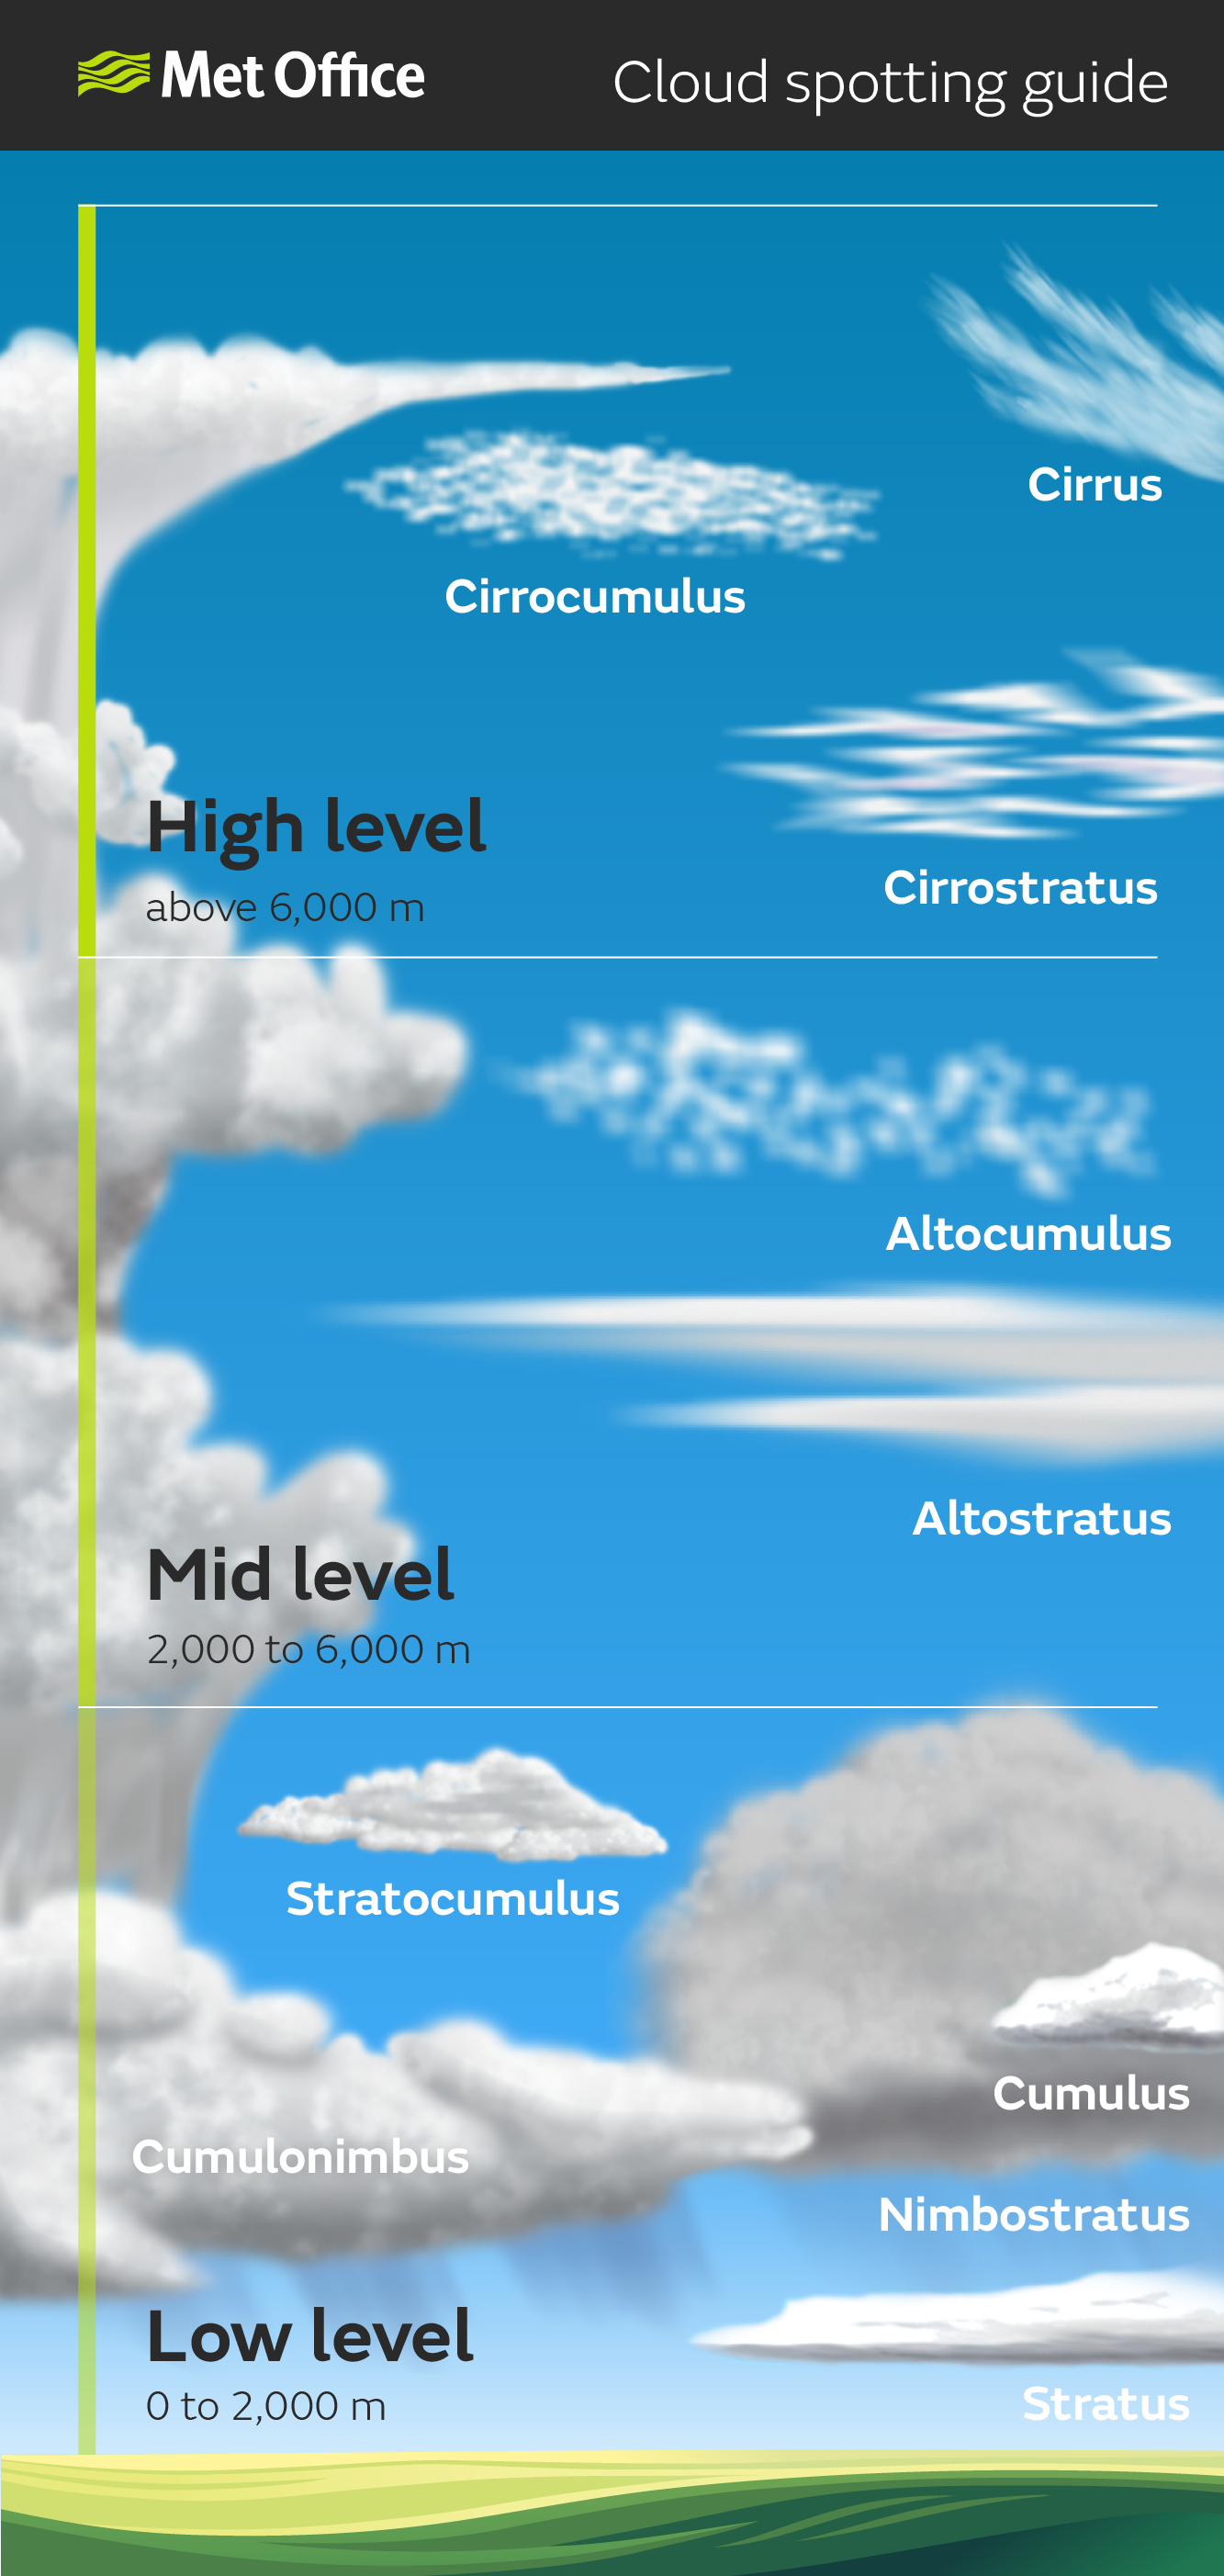
\includegraphics[height=10cm,keepaspectratio]{Cloud_infographic-01.png}
\caption{Schematische Darstellung der zehn Wolkengattungen vom britischen Met Office\cite{metoffice}}
    \label{fig:cloudtypes}
\end{figure}

Aufgrund der Ähnlichkeit einiger Klassen und der doch recht geringen Anzahl an Bildern im Vergleich zu der Anzahl an Klassen entschieden wir uns für eine Gruppierung in die vier Oberklassen \glqq Cirriform\grqq, \glqq Stratiform\grqq, \glqq Cumuliform\grqq, sowie \glqq Stratocumuliform\grqq, die in Tabelle \ref{table:oberklassen} beschrieben und in Abbildung \ref{fig:klassen} zu sehen sind.

\begin{figure}[h!]
	\subfigure[Cirriform]
	{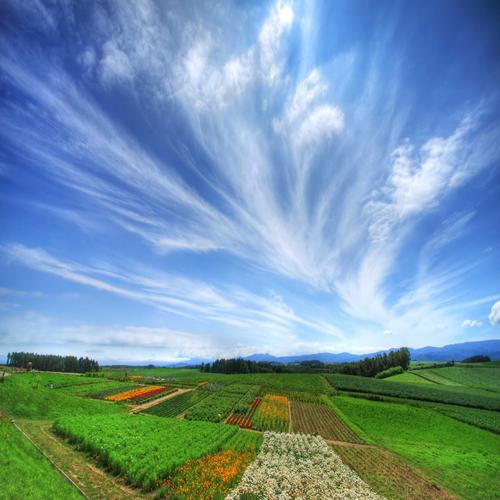
\includegraphics[width=0.53\textwidth]{cirriform7}}
	\subfigure[Stratiform]
	{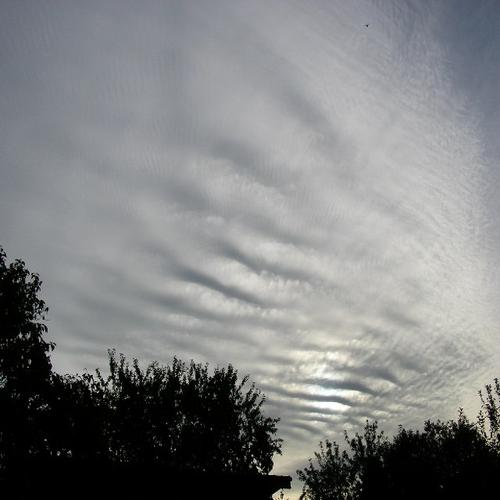
\includegraphics[width=0.53\textwidth]{stratiform30}}
	\\
	\subfigure[Cumuliform]
	{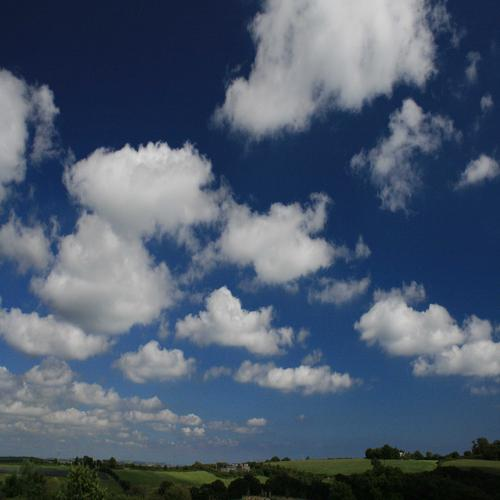
\includegraphics[width=0.53\textwidth]{cumuliform0}}
	\subfigure[Stratocumuliform]
	{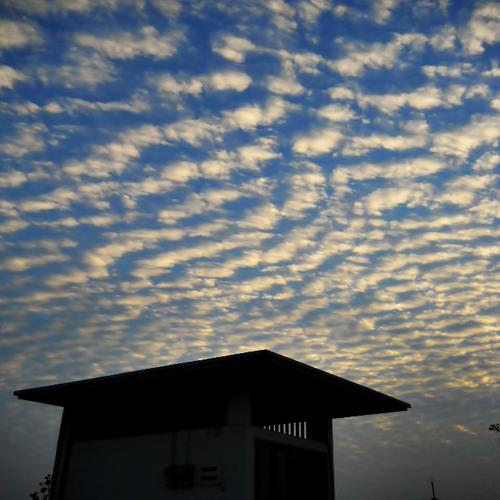
\includegraphics[width=0.53\textwidth]{stratocumuliform171}}
	\caption{Übersicht der vier Oberklassen}
	\label{fig:klassen}
\end{figure}


\begin{table}[h!]
\begin{tabular}{l | p{3.5cm} | p{3.5cm} | l}
    Hauptklasse & Unterklassen & Beschreibung & \# Bilder \\ \hline
    Cirriform & Cirrus & gefedert, oft durchsichtig; sehr dünn und gefächert & 123 \\ \hline
    Stratiform & Cirrostratus, Altostratus, Nimbostratus, Stratus & sehr flächig, zusammenhängend; meist durchgängige Bedeckung & 129 \\ \hline
    Cumuliform & Cumulus, Cumulonimbus & große Haufen, \glqq Schäfchenwolken\grqq & 294 \\ \hline
    Stratocumuliform & Cirrocumulus, Altocumulus, Stratocumulus & viele kleine Haufen über eine große Fläche & 287 \\
\end{tabular}
    \caption{Zusammensetzung und Beschreibung unseres Klassifizierungsschemas}
    \label{table:oberklassen}
\end{table}

Wie man auch schon an den Namen der verschiedenen Wolkengattungen sieht, gehen die Klassen leider teils ineinander über, was die Unterscheidung deutlich erschwert.
Außerdem gibt es noch sehr viele Arten, Unterarten und Begleitwolken, die sich teilweise ebenso in ihren Eigenschaften überschneiden.
Eine gute Übersicht der Wolkengattungen, -arten, etc. findet man in der \emph{Wikipedia} \cite{wiki:wolkenarten}.

\section{Methodik}
\label{sec:methodik}

% TODO: Methodik
%Hier sollte stehen, wie wir unser Problem lösen, sprich, wie unser Endsystem funktioniert.
%Warum machen wir es so und nicht anders?
%Wie funktionieren die Verfahren, die wir nutzen?

Im diesem Abschnitt erläutern wir die Methodik der beiden Klassifikationsansätze.
Eine Übersicht über den groben Ablauf kann in Abbildung \ref{fig:ablauf} gewonnen werden. 
Bevor mit der eigentlichen Klassifikation begonnen wird, werden die Ursprungsbilder zunächst möglichst so zugeschnitten, dass nur noch Himmel im Bild vorhanden ist (Abschnitt \ref{sec:vorverarbeitung}).

\begin{figure}
	\centering
	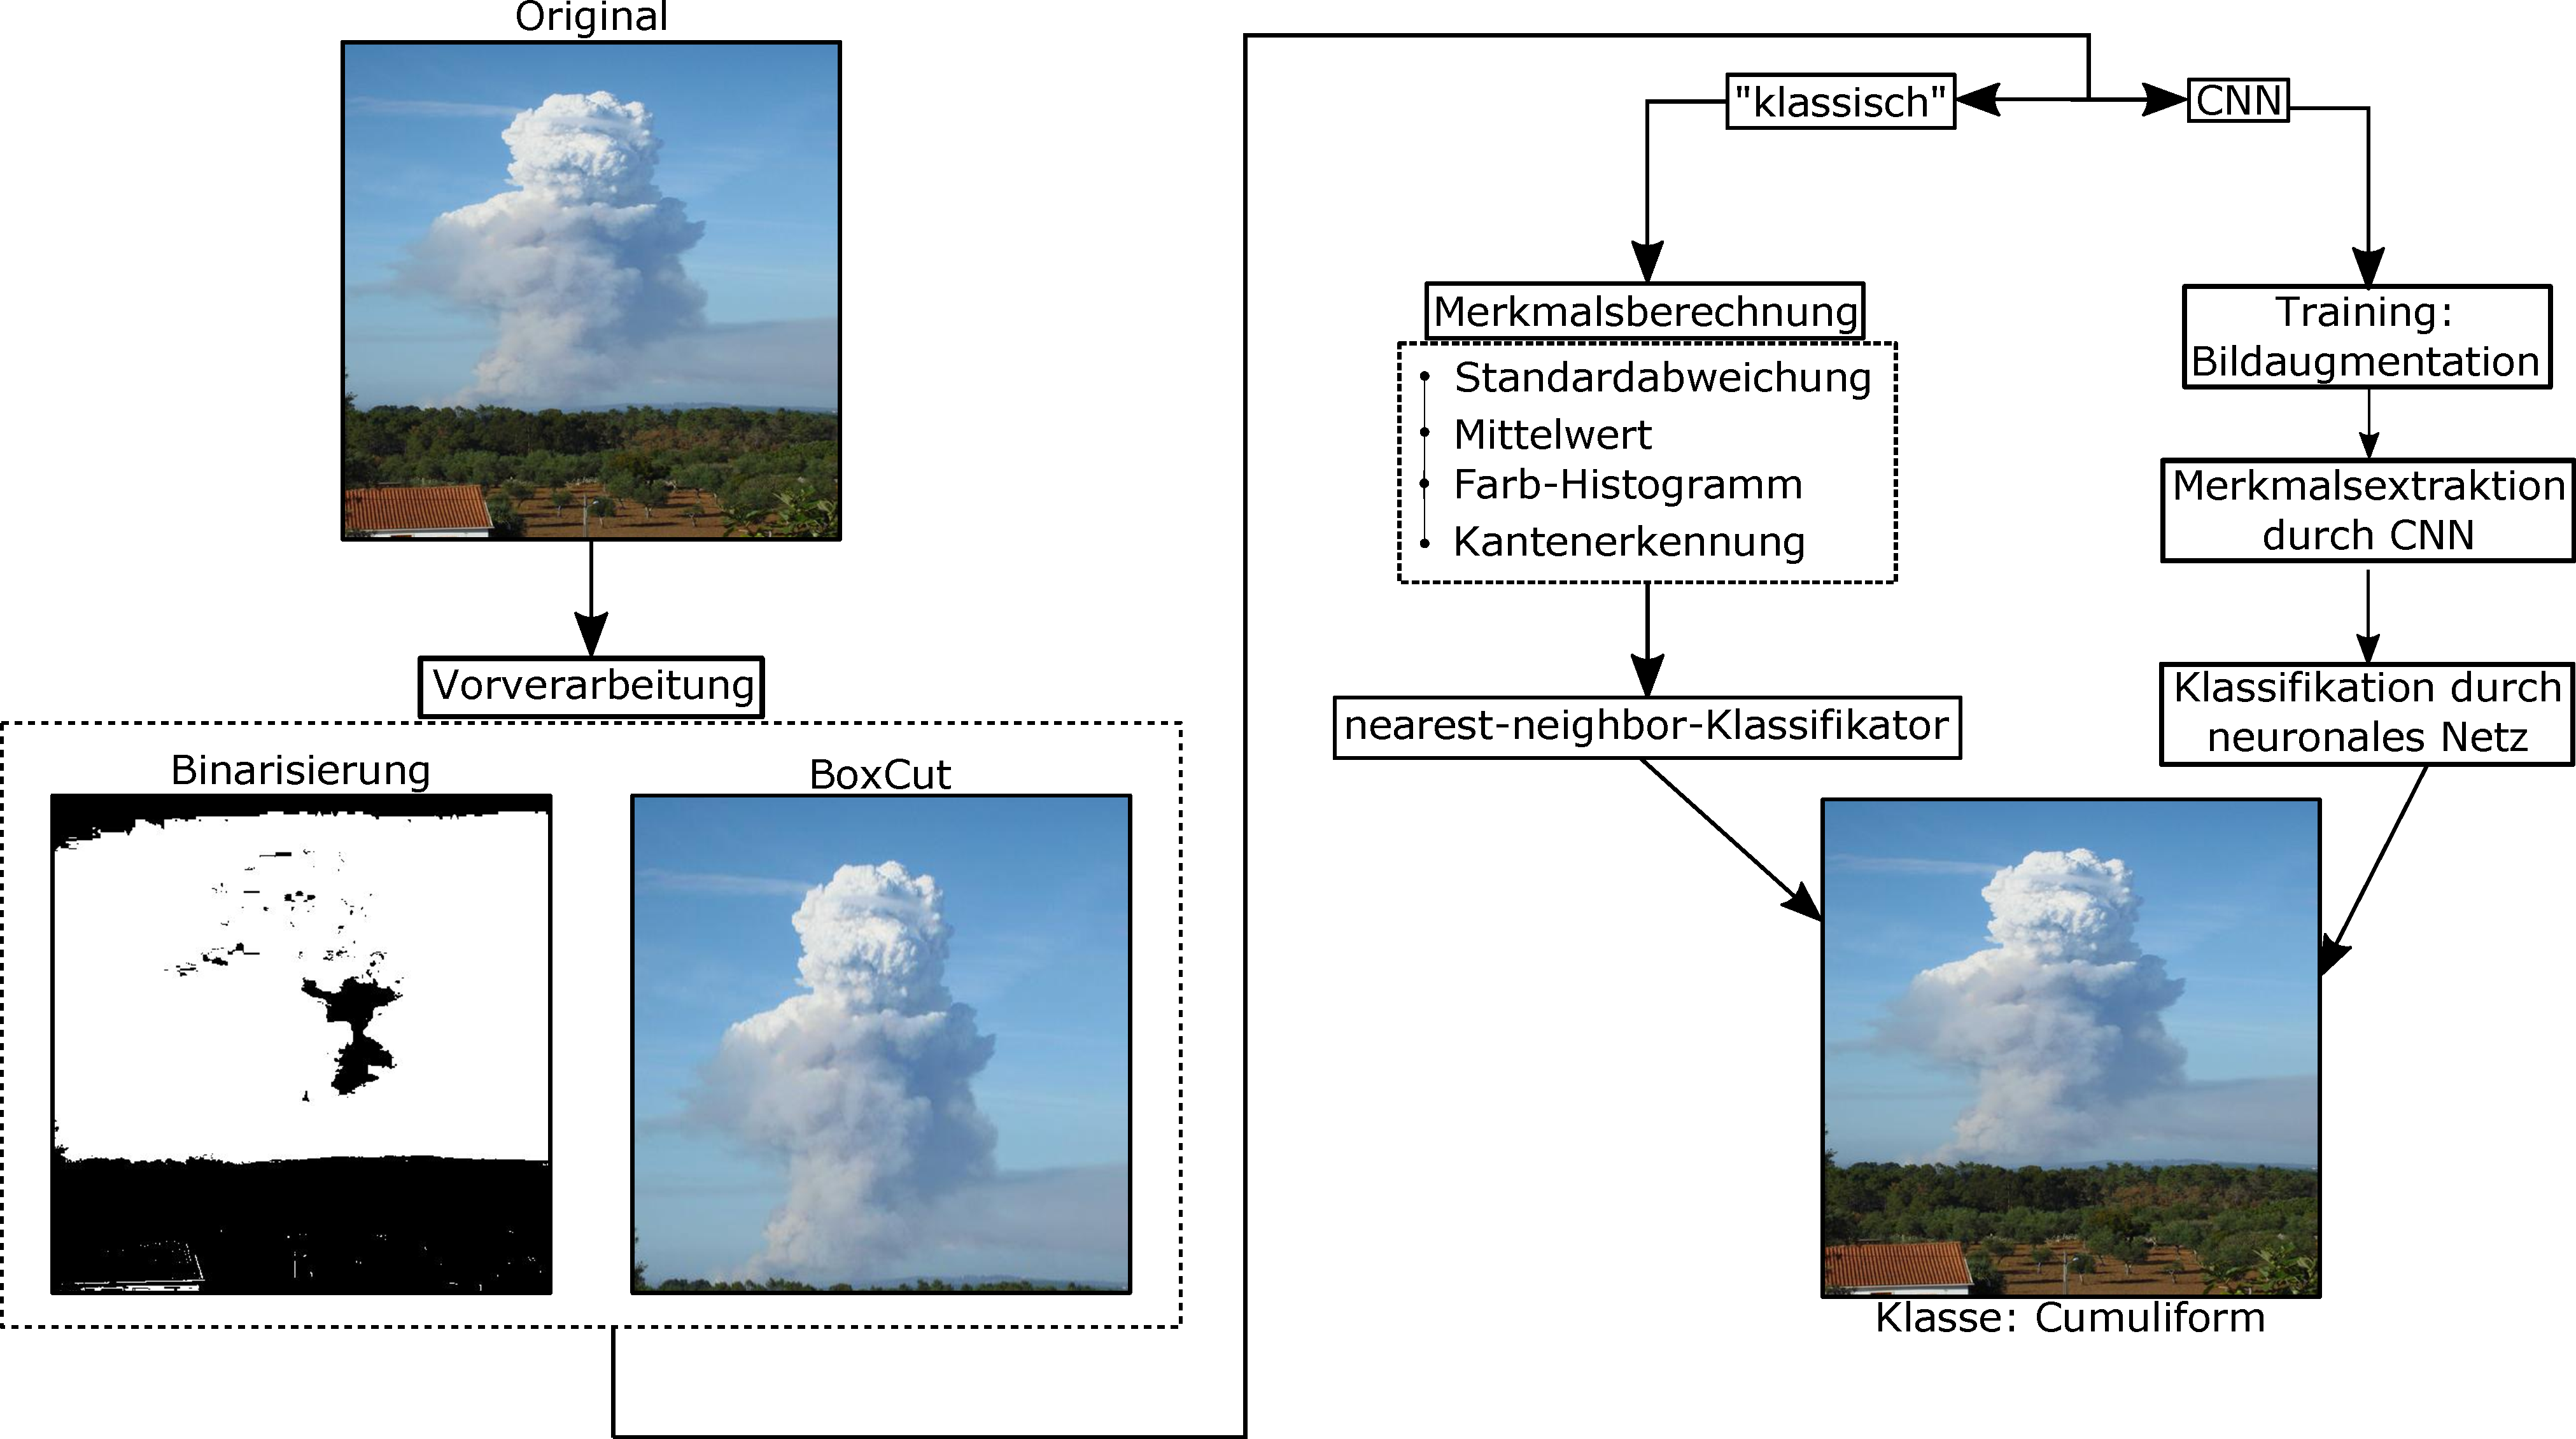
\includegraphics[height=0.25\paperheight]{Ablauf.pdf}
	\caption{Ablauf der Klassifikation}
	\label{fig:ablauf}
\end{figure}

Im \glqq klassischen\grqq\ Ansatz erfolgt hier nun die Bestimmung der Merkmale.
Neben den oft verwendeten Merkmalen Standardabweichung, Mittelwert und einem Farb-Histogramm wird auch eine Kantenerkennung durchgeführt (Abschnitt \ref{sec:kanten}).
Zum Schluss dieses Ansatzes nutzen wir nun einen \emph{nearest-neighbor}-Klassifikator, der die Merkmale des zu klassifizierenden Bildes mit denen der Bilder im Trainingsdatensatz vergleicht.
Der zugehörige Train/Validation-Split bei diesem Ansatz war 8:2. % TODO: Dieses Detail vielleicht woanders hin?

Beim auf Machine Learning basierten Ansatz wird im Training der doch recht kleine Datensatz durch Data Augmentation kompensiert (Abschnitt \ref{sec:augmentation}).
Es folgt die Merkmalsextraktion durch ein auf ImageNet vortrainiertes Convolutional Neural Network (CNN); die extrahierten Merkmale werden dann durch ein Klassifikationsnetz klassifiziert (Abschnitt \ref{sec:neural}).
% TODO: Training/Validation/Testing split?


\subsection{Vorverarbeitung der Bilder}
\label{sec:vorverarbeitung}
Da unsere ursprünglichen Bilder in ihren Dimensionen und in ihrer Art und Weise, wie sie entstanden sind sich stark unterscheiden, mussten wir sie vor der eigentlichen Klassifikation anpassen.
Zuerst haben wir unpassende Bilder, wie zum Beispiel von einem Sturm oder Fotos, auf denen die Wolken kaum erkennbar waren, manuell aussortiert.
Wie erwähnt war oft der untere Rand des Bildes nicht mehr nur reiner Himmel. Oft waren auch Wiesen oder Bäume zu erkennen, die der Klassifizierung Probleme bereiteten.
Durch eine Binarisierung und unter Anwendung unseres BoxCut Algorithmus, die in Kapitel \ref{sec:binary} und Kapitel \ref{sec:boxcut} näher erläutert werden, konnten wir relativ akkurat den Himmel vom restlichen Bild trennen.
Zum Schluss haben wir die Bilder noch auf die einheitliche Größe von 500x500 Pixel gebracht, bei welcher die Algorithmen noch schnell ein genaues Ergebnis berechnen konnten.

\subsubsection{Binarisierung} 
\label{sec:binary}
Die Binarisierung haben wir mithilfe des arithmetischen Mittels über das gesamte Bild sowie dem Farbwert und der Helligkeit aus dem HSV-Farbraum implementiert.
So gehört  ein Pixel dann zum Vordergrund, falls er heller ist als der Durchschnitt der Helligkeit des gesamten Bildes und falls er weder grün noch sehr stark dunkel ist.
Dies hat nach vielem herum experimentieren für ein gutes Ergebnis gesorgt. \ref{fig:boxAlg}.

\subsubsection{BoxCut Algorithmus}
\label{sec:boxcut}
Nach dem Binarisieren versucht der BoxCut Algorithmus den eigentlichen Himmel vom Rest des Bildes auszuscheiden. Dazu wird von unten eine rechteckige Fläche des Bildes ausgewählt. Die Höhe beträgt dabei ca. 10\%
des Bildes und die gesamte Breite (dargestellt durch das rote Rechteck im mittleren binarisierten Bild in \ref{fig:boxAlg}). In dem markierten Rechteck wird dann der durchschnittliche Farbwert berechnet.
Liegt dieser über unserem Schwellwert von 0.35 liegt, so gehört ein Teil der Box wahrscheinlich zum Himmel, sodass das Bild bis zum unteren Teil der Box geschnitten wird.
Falls aber der durchschnittliche Farbwert unter dem Schwellwert liegen sollte, so wird die Box um die Hälfte ihrer Höhe nach oben verschoben. Dies wird solange fortgeführt, bis letztlich der Schwellwert überschritten wird und das Bild zugeschnitten wird.


\begin{figure}[h!]
\centering
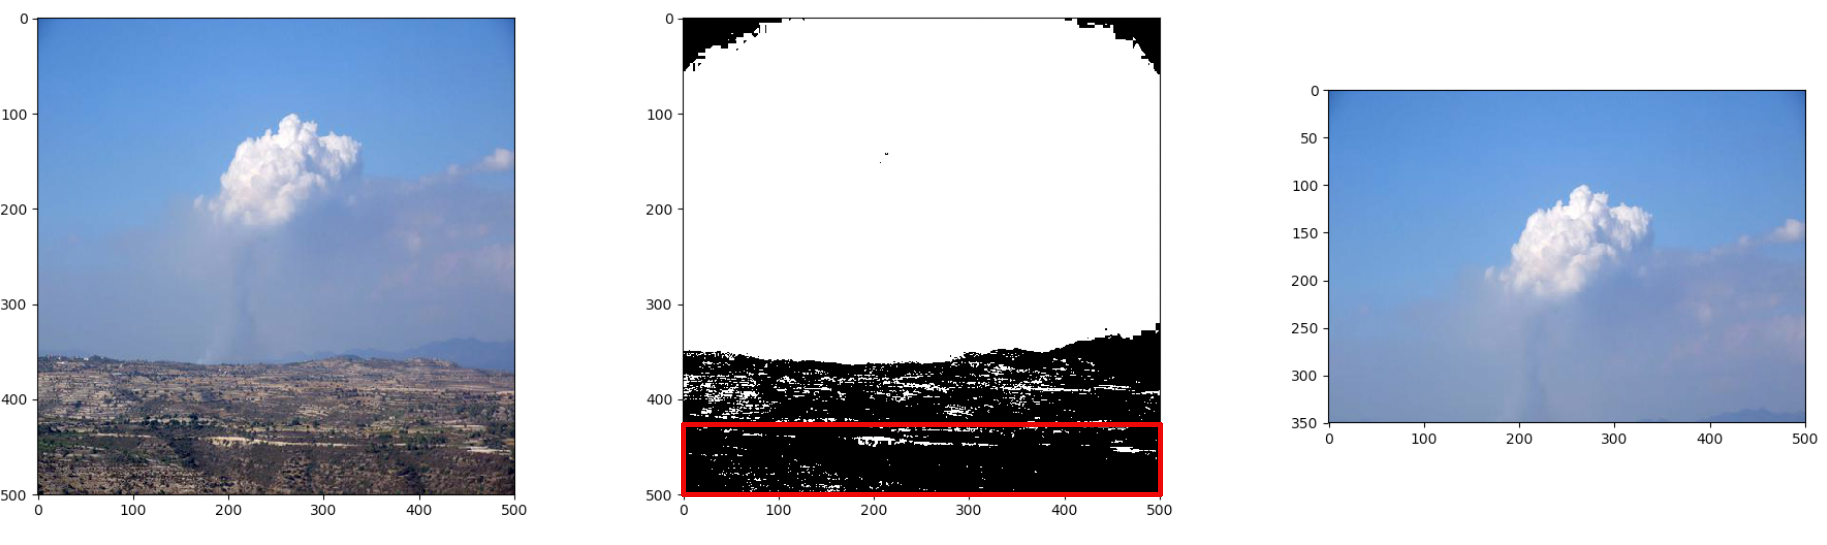
\includegraphics[width=1.1\textwidth]{boxAlg}
\caption{BoxCut-Algorithmus hat den Himmel erfolgreich von der Erde getrennt}
\label{fig:boxAlg}
\end{figure}


\subsection{Klassischer Ansatz}

% TODO: Es fehlt noch eine genauere Beschreibung des klassischen Ansatzes..., sprich, die finalen Ergebnisse, die im "Experimente"-Abschnitt beschrieben werden, sollten hier zusammengefasst stehen... oder zumindest so grob...

\subsubsection{Kantenzählung}
\label{sec:kanten}
Ein Merkmal, welches wir neben dem Mittelwert, der Standardabweichung und den Farb-Histogrammen verwenden, misst die Anzahl der Kanten auf den Bildern.
Dazu wird zuerst das Bild in ein Graustufenbild umgewandelt, da man somit nicht die Kanten für jeden Farbwert im RGB-Farbraum einzeln berechnet werden müssen. Als nächstes wird ein Gaussfilter mit Sigma = 2 auf das Bild angewendet, damit nur die gröberen Kanten ins Gewicht fallen. Danach wird mit Hilfe des Sobel-Filters ein Kantenbild erzeugt.
Dort, wo sich Kanten befinden, sind die Pixel heller, d.h. die Werte sind höher.
Diese Werte werden dann zeilenweise aufsummiert, sodass ein Histogramm wie auf dem rechten Bild in Abbildung~\ref{fig:kaz} entsteht. So können die Kanten pro Zeile von zwei Bildern verglichen werden.

\begin{figure}[h!]
\centering
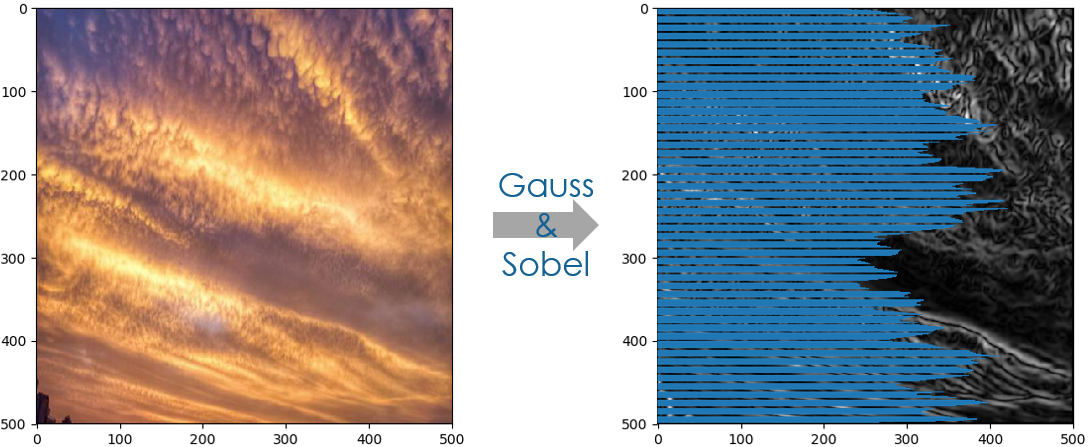
\includegraphics[width=\textwidth]{Kantenzaehlung.png}
\caption{Visualisierung der Kantenzählungs-Funktion}
    \label{fig:kaz}
\end{figure}


\subsection{Machine-Learning-Ansatz}

\subsubsection{Augmentation der Bilder}
\label{sec:augmentation}

Um trotz des recht kleinen Datensatzes akzeptable Ergebnisse zu erzielen, haben wir Data Augmentation eingesetzt.
Zuerst wurde jedes Original-Trainingsbild halbiert, sodass sich effektiv die Anzahl der Trainingsbilder verdoppelt.
Weiterhin wurde die in Keras verfügbare Data-Augmentation-Funktionalität genutzt, woduch im Training bilder zufällig gespiegelt, rotiert, geschert, sowie gezoomt wurden.
Beide Maßnahmen erhöhten die Genauigkeit des Endsystems deutlich.

Trainiert wurde auf 4096 Bildern---eine höhere Anzahl an Bildern brachte keine signifikante Genauigkeitsverbesserung.


\subsubsection{Merkmalsextraktion und Klassifizierung}
\label{sec:neural}

Bei der Merkmalsextraktion wurde darauf verzichtet, ein eigenes CNN zu konstruieren und zu trainieren.
Stattdessen verwenden wir, wieder aufgrund der geringen Datensatzgröße, ein in Keras vorhandenes, auf ImageNet vortrainiertes Netz.
Die Wahl fiel dabei auf \emph{Xception} \cite{xception}.
Wir wählten es aufgrund der (verglichen mit den anderen in Keras vorhanden Netzen) hohen Genauigkeit bzgl.\ ImageNet.\footnote{Zwar hat \emph{Xception} zum aktuellen Zeitpunkt nicht die höchste Genauigkeit---dieses Netz wäre \emph{InceptionResNetV2}, wobei dieses nur ca. einen Prozentpunkt besser abschneidet---ist aber 60\% kleiner als \emph{InceptionResNetV2} und auch deutlich performanter.}

Die von \emph{Xception} errechneten 2048 Merkmale wurden nun durch ein weiteres, von uns konstruiertes neuronales Netz konstruiert.
Hier folgen auf zwei Fully-connected Layer mit 128 Neuronen und ReLU-Aktivierung ein letzter Fully-connected Layer mit 4 Neuronen und Softmax-Aktivierung, die als Ausgabe dient.
Zwischen den Schichten wurden je 60\% der Verbindungen gekappt, um Overfitting vorzubeugen.

% TODO: Loss-Funktion (Categorical Crossentropy), Optimierer (SGD, Learning Rate 0.001, Momentum 0.9)
% TODO: Train/Validatoin/Test split (0.64/0.16/0.2)

In der Anwendung des Netzes auf Testfälle wurde nun der Input in drei verschiedene, sich teils überlappende, Segmente aufgeteilt (s. Abbildung \ref{fig:augmentation}), und die Klassifizierungspipeline dann auf jedes Segment angewendet, die dabei resultierenden Gewichte der Outputschicht summiert, und die Kategorie mit dem höchsten Gewicht als Klassifizierung gewählt.

\begin{figure}[h!]
\centering
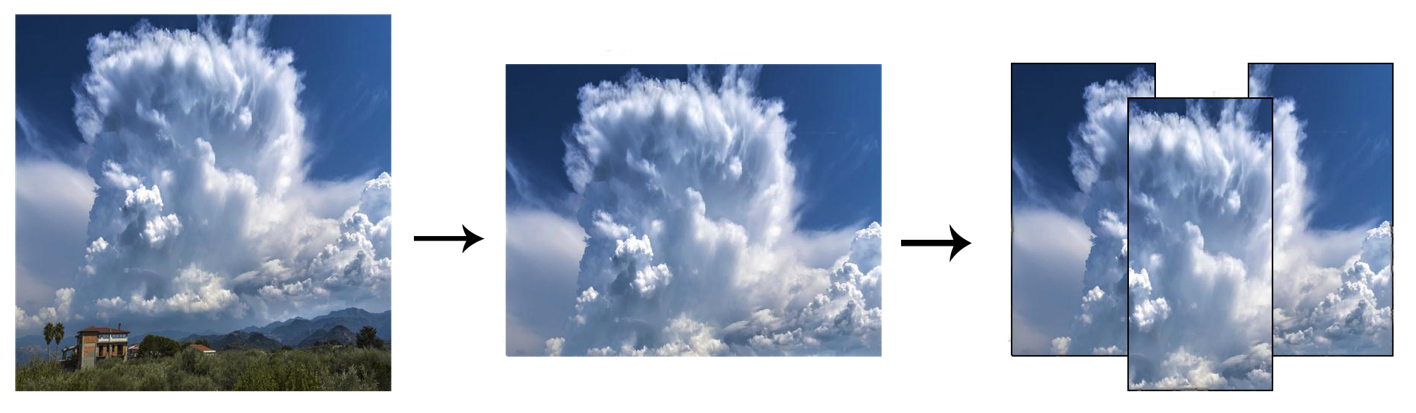
\includegraphics[width=\textwidth]{Augmentation}
\caption{Aus einem Originalbild werden drei verschiedene, aber sich überlappende Bilder}
    \label{fig:augmentation}
\end{figure}


\section{Experimente und Ergebnisse}
\label{sec:experimente}
In diesem Abschnitt werden die erzielten Ergebnisse unter verschiedenen Parametern vorgestellt.

\subsection{Klassischer Ansatz}%TODO: Daten bei Änderungen aktualisieren
Die höchste Genauigkeit, die wir mit dem klassischen Ansatz erzielen konnten, beträgt 49\%. Wie gut dabei die einzelnen Merkmale abschneiden, kann man aus Tabelle~\ref{tab:gen} herauslesen. Dabei steht \textit{mean} für den Mittelwert und \textit{std} für die Standardabweichung. 

\begin{table}[h]
\centering
\begin{tabular}{|l|l|l|l|l|l|l|}
 \hline
 \textbf{Merkmale:}&mean&std&1D-Hist.&3D-Hist.&Grau-Hist.&Kantenz.\\
 \hline
 \textbf{Erfolg:} & 28\% & 32\% & 35\% & 38\% & 35\% & 41\% \\
 \hline
\end{tabular}
\caption{Genauigkeit der einzelnen Merkmale, gerundet}
\label{tab:gen}
\end{table}

\begin{table}[h]
\centering
\begin{tabular}{|l|l|l|l|}
 \hline
 \textbf{Kombi.:}&mean+std&mean+std+Kantenz.&Kantenz.+3D-Hist.\\
 \hline
 \textbf{Erfolg:} & 40\% & 48\% & 49\% \\
 \hline
\end{tabular}
\caption{Genauigkeit von Merkmalskombinationen, gerundet}
\label{tab:gen2}
\end{table}

Abbildung~\ref{fig:meanstd} zeigt, dass die verschiedenen Klassen mithilfe von Mittelwert und Standardabweichung nur schwer auseinanderzuhalten sind und sich nicht leicht in verschiedene Klassen trennen lassen. Trotzdem erreichen wir hier nur mit diesen beiden Merkmalen eine Genauigkeit von 40\%.
\begin{figure}[h!]
\hspace*{-3cm}
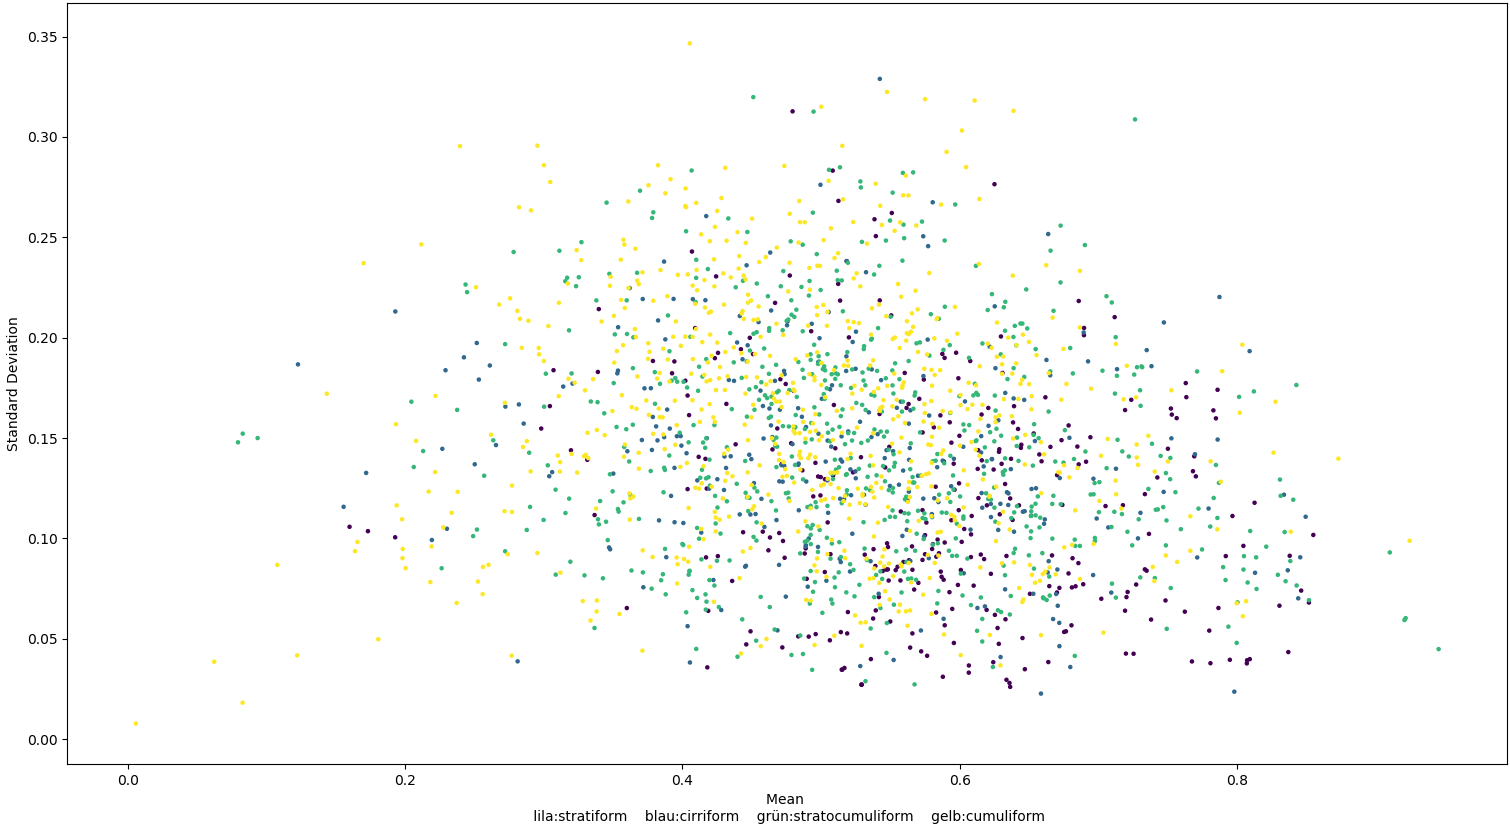
\includegraphics[width=1.5\textwidth]{Scatterplot_mean_std.png}
\caption{Scatterplot für Mittelwert und Standardabweichung}
\label{fig:meanstd}
\end{figure}

Bei der Kantenzählung wurden beim Gaussschen Weichzeichner verschiedene Sigma Werte ausprobiert, wobei sich Sigma = 2 als am besten herausstellte (siehe Tabelle~\ref{tab:sigma}).
Dies ist so, da bei größeren Sigmas die Kanten zu sehr verschwimmen %<-- Bin mir da nicht 100% sicher, ob das stimmt, weil ich nicht weiß, ob ich Sigma richtig verstanden habe... || so hätte ich das auch verstanden - Max; ich auch - alo
\begin{table}[h]
\centering
\begin{tabular}{|l|l|l|l|l|l|}
 \hline
 \textbf{Sigma:} & 0 & 1 & 2 & 3 & 4\\
 \hline
 \textbf{Erfolg:} & 40\% & 41\% & 41\% & 36\% & 35\% \\
 \hline
\end{tabular}
\caption{Genauigkeit der Kantenzählung bei verschiedenen Sigmas für den Weichzeichner}
\label{tab:sigma}
\end{table}

Die Kantenzählung war besonders darauf ausgelegt, stratiforme Wolken %(flächige Wolken)
zu identifizieren, da diese meist durchgängige Flächen sind und daher wenig Kanten haben.
Abbildung~\ref{fig:kbs} zeigt einen Boxplot und einen Swarmplot für die Kantenzählung.
Dabei ist wichtig zu berücksichtigen, dass für die Plots die Histogramme auf einen Wert reduziert wurden, das heißt der Plot spiegelt das Merkmal nur annäherungsweise wieder.
Während der Boxplot vermuten lässt, die stratiformen Wolken ließen sich mithilfe des Merkmals alleine klar von den anderen trennen, zeigt der Swarmplot, dass dies nur für etwa die Hälfte der Bilder mit stratiformen Wolken gilt. %Also haben wir das Merkmal so für unseren Entscheidungsbaum verwendet, dass wir alle Wolken die einen Gesamtkantenwert von unter 1000 haben als stratiform klassifizieren, dabei aber nicht ausschließen, dass unter den Verbliebenen noch stratiforme Wolken sind...könnte man hier schreiben wenn wir es machen. -- 

\begin{figure}[h!]
\centering
\subfigure[Boxplot Kantenzählung]
{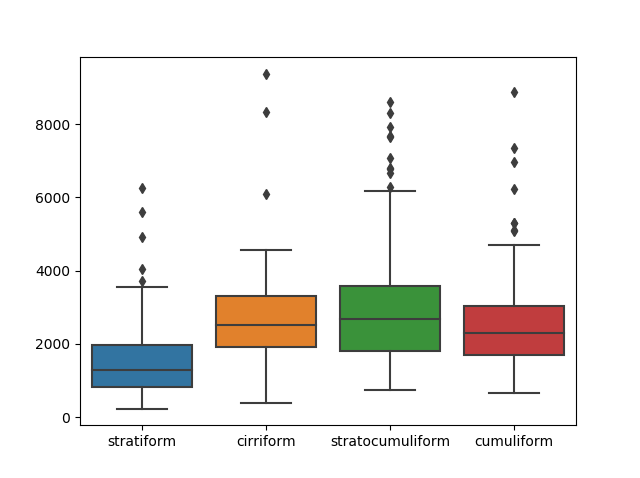
\includegraphics[width=0.83\textwidth]{edge_count_boxplot1.png}} \\
\subfigure[Swarmplot Kantenzählung]
{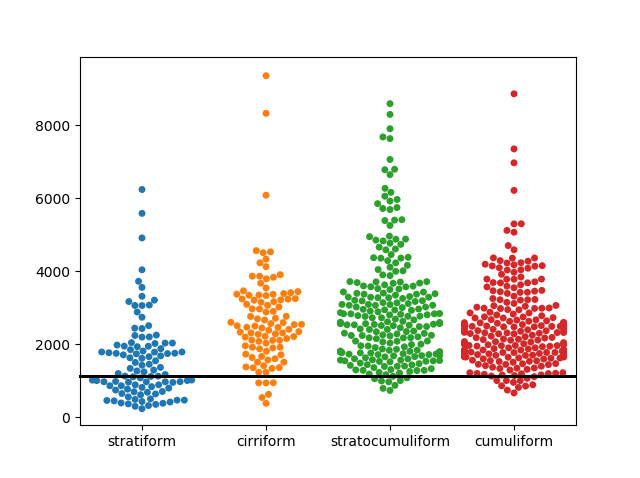
\includegraphics[width=0.83\textwidth]{edge_count_swarmplot1.png}}
\caption{Unterschiede in den Kantenzählungswerten pro Klasse}
    \label{fig:kbs}
\end{figure}



\subsection{Gescheiterte Ansätze}
Wir hatten noch zusätzliche Merkmale implementiert, die nicht gut genug funktioniert haben, um sie zu verwenden.
Ein Ansatz war es das Region Growing anzuwenden, um so aus den Bildern die Zusammenhangskomponenten der Wolken auszuscheiden oder auch um die Frequenzen der Regionen aus diesen abzuleiten.
Besonders bei der Klassifizierung von Cumuluswolken
wäre die Anzahl der Zusammenhangskomponenten sehr aussagekräftig gewesen.
Wir konnten das Region Growing leider nicht mit unseren Daten verwenden, da auf vielen Bildern die Wolken ineinander übergehen und trotz Runterskalierung auf 50p x 50p, die Berechnung pro Bild noch immer bis zu 30 Sekunden gedauert hat.


\subsection{Neuronale Netze}

Unser auf neuronalen Netzen basierendes System erreichte eine Klassifizierungsgenauigkeit von 65.6\% auf einem aus 20\% des Datensatzes bestehendem Testdatensatz, der kein Bild mit dem Trainingsdatensatz gemeinsam hat.

Aus der Konfusionsmatrix (Tabelle \ref{tab:confusionNeural}) ist zu erkennen, dass cumuliforme Wolken besonders gut erkannt werden, und cirriforme Wolken vergleichsweise schlecht.
Weiterhin wird ein recht hoher Anteil an Bildern fälschlicherweise als stratocumuliform klassifiziert (besonders cirriforme Wolken), ähnliches gilt für cumuliforme Wolken.

Wir vermuteten, dass dies an der recht ungleichen Verteilung der verschiedenen Labels im Datensatz liegt (siehe Tabelle \ref{table:oberklassen}).
Ein erneuter Testdurchlauf nach Angleichen der Klassengrößen durch entfernen von Bilderns aus überrepräsentierten Klassen bestätigte diese Vermutung.
Im Allgemeinen sank zwar die Genauigkeit deutlich (um ca. 8 Prozentpunkte), jedoch verschwanden die beschriebenen Anomalien.
Aufgrund des allgemeinen Genauigkeitsverlust, und da auch in Alltag die Wolkenformen eher so verteilt sind wie im ursprünglichen Datensatz, entschieden wir uns dafür, diesen unverändert beizubehalten.
% TODO: Auch hierfür eine Konfusionsmatrix... ich habe die Daten verloren, vielleicht lasse ich das System morgen nochmal laufen, sonst muss das so "mündlich" beschrieben reichen. -- Lukas

% TODO: Wie schnell sind unsere Verfahren?
%Was passiert, wenn man einzelne Teile des Systems austauscht oder Merkmale entfernt (dies evtl.\ auch mit Diagrammen zeigen)?
%Wie wirken sich Änderungen der Parameter/Hyperpara\-meter auf die Ergebnisse aus?

\begin{table}
    \begin{tabular}{| l | l | l | l | l |}
        \hline
        Label & cir & cum & str & str-cum \\ \hline
        Cirriform (cir) & 40\% & 14\% & 2\% & 44\% \\ \hline
        Cumuliform (cum) & 2\% & 81\% & 2\% & 15\% \\ \hline
        Stratiform (str) & 5\% & 18\% & 56\% & 21\% \\ \hline
        Stratocumuliform (str-cum) & 9\% & 24\% & 4\% & 64\% \\ \hline
    \end{tabular}
    \caption{Konfusionsmatrix des auf neuronalen Netzen basierenden Klassifikators. Zeilen sind die wirklichen Labels, Spalten die vom Klassifikator errechneten Labels. 80\% heißt, dass 80\% der Bilder mit dem gegebenen echten Label das gegebenen errechnete Label haben}
    \label{tab:confusionNeural}
\end{table}

\subsection{Menschen klassifizieren Wolken}

Da uns aufgefallen ist, dass es nicht nur für den Computer sondern auch für uns schwierig ist, die Wolken zu klassifizieren, haben wir uns dazu entschieden, eine kleine Studie durchzuführen.
Bei dieser Studie sollten die sechs Probanden jeweils sechzehn Wolkenbilder in unsere vier Kategorien einteilen.
Sie haben die Übersicht aus Abbildung~\ref{fig:cloudtypes} bekommen und pro Klasse sechs Trainingsbilder als Referenz.
Dabei wurde eine durchschnittliche Genauigkeit von 51\% erreicht. Der Versuchsaufbau und die Ergebnisse sind noch einmal genauer im "CloudGame.pdf" im Anhang geschildert.

Die erreichte Genauigkeit von 51\% ist sehr nah an dem Ergebnis unseres klassischen Ansatzes dran, liegen überraschenderweise jedoch unter den Ergebnissen des Maschine-Learning-Ansatzes.
Zu beachten ist jedoch, dass die 36 Bilder, welche für die Testpersonen gewählt wurden, gut klassifizierbare Bilder waren.
Im Allgemeinen ist also damit zurechnen, dass ungeschulte Menschen noch schlechter abschneiden.

\section{Fazit}
\label{sec:fazit}

% Fazit
%Was ist unser Fazit?
%Zusammenfassung und Einordnung unserer Ergebnisse.
%Ausblick?

Insgesamt können wir sagen, dass es eine Herausforderung war, die verschiedenen Bilder zu klassifizieren.
Nicht nur innerhalb einer Wolkenart unterscheiden sich die Bilder teils sehr stark voneinander, auch ist es vor allem die Ähnlichkeit vieler Bilder in jeweils verschiedenen Wolkenklassen, die die korrekte Klassifizierung der Wolken erschwert.
Und da es sogar für Menschen schwer ist, viele Bilder ihrer richtigen Kategorie zuzuordnen, hatten wir besonders bei der klassischen Methode nichtall zu genaue Ergebnisse erwartet.
Allerdings sind wir mit 49\% für die klassische Methodik schon sehr zufrieden, da dies noch weit besser ist, als ein zufälliges Zuordnen der Klassen.

Auch beim auf neuronalen Netzen aufbauenden Ansatz waren wir von der erreichten Leitung positiv überrascht, besonders in Hinblick auf den recht kleinen Datensatz.
Sofern sich die in der Entwicklung festgestellte Beziehung zwischen Datensatzgröße und erreichter Genauigkeit fortsetzt, wäre eine Leistung jenseits der 75\% nicht überraschend.
Weiterhin wäre es dann interessant, das zur Merkmalsextraktion genutzte CNN vollständig selbst zu trainieren; dies hatte die aktuelle Datensatzgröße nicht zugelassen.

Ebenso können wir uns vorstellen, dass ein viel besseres Ergebnis zu erreichen ist, wenn die Bilder alle nach einer bestimmten Norm aufgenommen wären, zum Beispiel mit dem selben Winkel zum Himmel, bei gleicher Helligkeit oder aber vom selben Standpunkt aus.
Jedoch sind dann auch deutliche Verluste bzgl.\ der Generalisierbarkeit auf andere Situationen zu erwarten.
% TODO?: vvvv ich kann aus dem referenzierten Paper nicht erkennen, was da mit Overfitting ist. -- Lukas
% Allerdings müsste man dann äußerst vorsichtig sein, wie im Falle der Kieler Universität, das die Bilder so nicht zum overfitten der Ergebnisse führen.\cite{heinle}

\bibliographystyle{babplain}
\bibliography{bibliography}

\end{document}

